\documentclass{article}
\usepackage{graphicx} % Required for inserting images
\usepackage{amsmath}
\usepackage{float}
\usepackage{minted}

\title{Algorithms and Data Structures - Exam Notes}

\date{Spring 2024}

\setminted[python]{breaklines, framesep=2mm, fontsize=\footnotesize, numbersep=5pt}

\begin{document}

\maketitle

\tableofcontents

\pagebreak

\section{Analysis of Algorithms}

\subsection{Order of Growth, from smallest to largest}

\begin{enumerate}
    \item $O(1)$
    \item $O(\log n)$
    \item $O(\sqrt n)$
    \item $O(\log (n) \sqrt n)$
    \item $O(n)$
    \item $O(n \log n)$
    \item $O(n^2)$
    \item $O(2^n)$
    \item $O(n!)$
    \item $O(n^n)$
\end{enumerate}

\subsection{Exam Questions}

\subsubsection{Asymptotic Equivalence ($f(N) \tilde g(N)$)}

\begin{enumerate}
    \item \textbf{Identify the dominant term} in each function. This is the term that grows the fastest as $N$ increases
    \item \textbf{Compare the leading coefficients} if the dominant terms are the same type in both functions
    \item \textbf{Eliminate options} where 2. is not satisfied
    \item \textbf{Check for simplification} where non-dominant terms become negligible at large $N$
    \item \textbf{Select the correct option} where the dominant terms (including the coefficients) match closely
    
\end{enumerate}

\subsubsection{Big-O Notation ($f(N)=O(g(N))$)}

\begin{enumerate}
    \item \textbf{Identify the highest order term} for both $f(N)$ and $g(N)$
    \item \textbf{Compare growth rates} of these terms. $f(N)$ should not exceed $g(N)$ by more than a constant factor as $N$ becomes very large
    \item \textbf{Eliminate options} where 2. is not satisfied
    \item \textbf{Select the correct option} by considering how each $f(N)$ behaves relative to $g(N)$ at large values of $N$
\end{enumerate}

\subsubsection{Code Analysis for Loops and Recursions}

\begin{enumerate}
    \item \textbf{Understand the structure of the loops and recursion}
    \item \textbf{Count iterations}:
    \begin{itemize}
        \item For loops: Calculate how many times the loop will execute relative to $N$
        \item For recursion: Determine how the recursion tree grows and estimate the total number of calls relative to $N$
    \end{itemize}
    \item \textbf{Estimate the total operations performed} based on the loops and recursive calls
    \item \textbf{Choose the smallest correct estimate} of complexity from the provided options
\end{enumerate}

\begin{itemize}
    \item \textbf{Note:} If a loop contains something like if $i < 5, j = N * N$, where $j$ is used in a nested loop, it's safer to account for it when choosing the smallest $O(...)$ estimate 
\end{itemize}

\subsubsection{Cost Models in Data Structures}

\begin{enumerate}
    \item \textbf{Identify the data structure} and read through the relevant methods
    \item \textbf{List possible costs} like array accesses, computations, or variable manipulations
    \item \textbf{Select the most fitting cost model} based on which operations are most frequent and critical in affecting performance
\end{enumerate}

\subsubsection{Recurrence Relations in Recursive Algorithms}

\begin{enumerate}
    \item \textbf{Analyze the base cases} to understand when recursion stops
    \item \textbf{Identify the operations} in the current call
    \item \textbf{Identify the recursive calls} and their conditions
    \textbf{Set up a recurrence} based on how each recursive call contributes to the total number of operations
    \item \textbf{Choose the smallest correct estimate} that fits the growth of operations dictated by the recursive structure, don't forget about 2.
\end{enumerate}

\textbf{Pattern-matching approach}: the answer should have:
\begin{itemize}
    \item A constant equivalent to the number of arithmetic operations in the function
    \item T() calls equivalent to the number of recursive calls in the function, with corresponding parameters
\end{itemize}

For example:

$r(N-1) \cdot r(N-2) + N$ is $T(N-1) + T(N-2) + 4$

A T() call should only ever be multiplied by a constant $a$ if it's called $a$ amount of times with the same parameters in the function.

\subsubsection{Running Time Analysis of a Repeated Method Call}

\begin{enumerate}
    \item \textbf{Analyze function complexity} determine the per-call complexity of the function
    \item \textbf{Examine loop execution} analyze how many times the function is called within the loop relative to $N$
    \item \textbf{Calculate total complexity} multiply the per-call complexity by the number of times the function is called
\end{enumerate}
\begin{itemize}
    \item If the function has a separate worst-case and amortised running time, consider how often it's called: use the amortised running time if it's called frequently within a loop, but rely on the worst-case scenario if it's seldom called (e.g., always \(\leq 5\) times, regardless of \(N\)).
    \item If the function has a string concatenation, remember that it takes time proportional to the length of the resulting string (in both Python and Java)
    \item Remember: amortisation doesn't carry over, so if you use the amortised running time for f(...), that does not mean you have to say that the loop has amortised running time
\end{itemize}

\section{Sorting Algorithms}

\begin{itemize}
    \item Sorting involves comparing and exchanging items, using minimal extra memory
    \item The efficiency of sorting algorithms is measured by counting compares and exchanges
    \item The algorithms work with any data type that can be compared with total order
    \item Total order means that comparisons are:
    \begin{itemize}
        \item \textbf{Reflexive}: for all $v$, $v=v$
        \item \textbf{Antisymmetric}: for all $v$ and $w$, if ($v<w$) then ($w>v$); and if ($v=w$) then ($w=v$)
        \item \textbf{Transitive}: for all $v$, $w$, and $x$, if ($v\leq w$) and ($w \leq x$), then $v \leq x$
    \end{itemize}
\end{itemize}

\subsection{Selection Sort}

\begin{itemize}
    \item Works by dividing the list into two parts: a sorted section at the beginning and an unsorted section for the rest
    \item Initially, the sorted section is empty, and the unsorted section is the entire list. The algorithm repeatedly:
    \begin{itemize}
        \item Selects the smallest element from the unsorted section
        \item Moves it to the end of the sorted section.
    \end{itemize}
    \item In-place sort, requiring no extra storage
\end{itemize}

\subsection{Insertion Sort}

\begin{itemize}
    \item Involves two sections of the array: the sorted section, which initially contains just the first element, and the unsorted section, which contains the rest
    \item The algorithm picks each element from the unsorted section and finds its correct position in the sorted section, shifting the larger sorted elements to the right to make room
    \item In-place sort, requiring no extra storage
\end{itemize}

\subsection{Merge Sort}

\begin{itemize}
    \item A divide-and-conquer algorithm
    \item Breaks down a list of items into smaller sub-lists, then merges them back together in sorted manner
    \item Operates in divide phase and a conquer phase
    \begin{itemize}
        \item During divide phase, list of items repeatedly divided in half until each sub-list consists of only one item
        \item During conquer phase, sub-lists combined back together in a sorted manner by comparing the first elements of the sub-lists and merging them back together in order
        \begin{itemize}
            \item While the 2 sub-lists aren't empty, compare the 2 first elements, and add the smaller one to the combined list
        \end{itemize}
    \end{itemize}
\end{itemize}

\subsection{Quick Sort}

\begin{enumerate}
  \item \textbf{Shuffle the Array:} Randomly shuffle the array to ensure performance guarantees, avoiding the worst-case scenario of $O(n^2)$ time complexity.
  \item \textbf{Choose a Pivot:} Typically, the first element of the array is chosen as the pivot ($a[lo]$).
  \item \textbf{Initialize Indices:} Set two pointers, $i$ starting from the left (after the pivot) and $j$ starting from the right end of the array.
  \item \textbf{Move Indices:}
    \begin{itemize}
      \item Move $i$ rightward until an element greater than or equal to the pivot is found.
      \item Move $j$ leftward until an element less than or equal to the pivot is found.
    \end{itemize}
  \item \textbf{Check and Swap:}
    \begin{itemize}
      \item If $i$ is less than $j$, swap $a[i]$ and $a[j]$. Repeat step 4.
      \item If $i$ is greater than or equal to $j$, break the loop.
    \end{itemize}
   \item \textbf{Final Swap:} Swap the pivot element ($a[lo]$) with the element at index $j$.
    \item \textbf{Recursively Sort the Subarrays:} 
    \begin{itemize}
      \item Recursively apply steps 2 to 6 to the subarray left of $a[j]$.
      \item Recursively apply steps 2 to 6 to the subarray right of $a[j]$.
    \end{itemize}
\end{enumerate}


\subsection{Radix Sort}

\subsubsection{LSD}

\begin{itemize}
    \item Sort each digit/char independently, from rightmost digit towards left
    \item Only works on strings/sequences of the same length
\end{itemize}

\subsubsection{MSD}

\begin{enumerate}
    \item Just like LSD, but sort from leftmost digit/char towards the right
    \item Works on strings/sequences of different lengths
\end{enumerate}

\section{Data Structures}

\subsection{Union Find (Disjoint Set)}

\begin{itemize}
    \item Keeps track of elements which are set into one or more disjoint sets
    \item Two primary operations: \textbf{find} and \textbf{union}
    \begin{itemize}
        \item Find tells you what set the element belongs to - returns root by following the parent nodes until a self loop is reached
        \item Union merges two sets together - finds root node of each component, if they are different make one the parent of the other
    \end{itemize}
    \item With an array implementation:
    \begin{itemize}
        \item Bijection - each object is given a unique mapping to an integer $[0,n[$
        \item At each index, the value is $i$'s root/parent
        \item During a union operation, either choose new parent arbitrarily, or in weighted union find, attach the smaller tree to the larger one
    \end{itemize}
    \item Path compression makes objects point directly to their root node - when finding the root of an element, path compression makes every other node in the path point directly to the root, thereby reducing the path length for future operations
\end{itemize}

\subsection{Stacks and Queues}

\subsubsection{Linked Lists}

\begin{itemize}
    \item Used to store collections of elements in sequential manner
    \item Each node contains a link to the next node in the sequence
    \item Efficient for insertion/deletion of elements, as these operations don't require shifting elements, just reassigning links
    \item Dynamically sized, can grow or shrink in size dynamically unlike arrays
    \item However, you can't directly access elements by their position, to access an element, you must traverse the list
    \item Also, each node required extra memory for the link
    \item Doubly linked lists have links to next and previous nodes
\end{itemize}

\subsubsection{Stacks}

\begin{itemize}
    \item Last-in-first-out
    \item Methods:
    \begin{itemize}
        \item \textbf{Push}: Add an element to the top of the stack
        \item \textbf{Pop}: Remove and return the element at the top of the stack
        \item \textbf{Is empty}: Check if the stack is empty
    \end{itemize}
    \item Can be implemented as linked list or array, but often linked list is more efficient
\end{itemize}

\subsubsection{Queues}

\begin{itemize}
    \item First-in-first-out
    \item Very similar to stack
    \item In linked list implementation, keeps track of last (tail) element, and push links the tail to the new element, rather than adding it to the head
\end{itemize}

\subsection{Priority Queues}

\begin{itemize}
    \item A priority queue is a data type that operates similar to a normal queue except that each element has a certain priority
    \item Elements must be comparable, so it must be able to be ordered in ascending/descending order 
    \item Methods:
    \begin{itemize}
        \item \textbf{Add}: Add an element to the queue
        \item \textbf{Poll}: Remove and return smallest/largest element in queue
        \item \textbf{Peek}: See smallest/largest element in queue
    \end{itemize}
    \item Priority queues often use heaps
\end{itemize}

\subsubsection{Binary Heaps}

\begin{itemize}
    \item A binary heap is a complete binary tree, which means it is perfectly balanced, except possibly for the last row, which is filled from left to right
    \item This structure ensures that the heap remains as compact as possible, minimizing the number of levels and thus the paths from any node to the root
    \item There are two types of binary heaps:
    \begin{itemize}
        \item \textbf{Min-Heap}: In a min-heap, the value of each node is less than or equal to the values of its children. The root, therefore, contains the minimum element of the heap.
        \item \textbf{Max-Heap}: In a max-heap, the value of each node is greater than or equal to the values of its children. The root contains the maximum element of the heap.
    \end{itemize}
    \item Operations:
    \begin{itemize}
        \item \textbf{Insertion}: New elements inserted on the bottom row, from left to right - when using an array, just insert it at the end. Then, they "bubble up" (swap with parent) until the heap invariant is satisfied
        \item \textbf{Polling} (in array):
        \begin{itemize}
            \item We swap a[0] (root) with last element, then remove and return it
            \item We "bubble down" the new root - swap with smallest (or largest in max heap) children, left node if tie, until heap invariant is satisfied
        \end{itemize}
        \item \textbf{Removal} (in array):
        \begin{itemize}
            \item Perform linear scan of elements until element to be removed is found, mark $i$
            \item Swap it with the last element, then remove and return in
            \item Bubble up what used to be the last element, now at $i$, until the heap invariant is satisfied
        \end{itemize}
    \end{itemize}
    \item To speed up removal, we can use a hash table to keep track of elements' indices; instead of doing a linear scan, we lookup the position in the table
    \item In a binary heap represented by an array (as it often is), the element at index $i$ usually has it's children at indices $2i$ and $2i+1$ (assuming 1-based indexing, other formats exist, such as 0-based, where it's $2i+1$ and $2i+2$)
    \item We can use a heap to perform heap-sort: add all elements from array to heap, then poll all elements from heap (and add them to array), until the heap is empty. This will result in an ordered array
\end{itemize}

\subsection{Hash Tables}

\begin{itemize}
    \item A hash table is a data structure that provides a mapping from keys to values using a technique called hashing. Keys must be unique, but values can be repeated
    \item A hash function $H(x)$ is a function that maps an immutable key '$x$' to a whole number in a fixed range
    \item A hash function $H(x)$ must be deterministic
    \item If $H(x)=H(y)$ then objects $x$ and $y$ might be equal, but if $H(x) \ne H(y)$ then $x$ and $y$ are certainly not equal
    \item A hash collision is when two objects $x$, $y$ hash to the same value ($H(x)=H(y), x \ne y$)
    \item Uniform hash functions are optimal to minimize the number of hash collisions
    \item $O(1)$ average insertion/removal/search complexity
    \item $O(n)$ worst-case i/r/s complexity
    \item Hash tables only have one entry per key, the same key is inserted again the existing value is updated
\end{itemize}

\subsubsection{Separate Chaining}

\begin{itemize}
    \item Deals with hash collisions by maintaining a data structure (usually a linked list) to hold all the different values hashed to a particular value
    \item In the linked list implementation, each object stores the key, value, and next object (or null pointer)
    \item To maintain $O(1)$ insertion/lookup complexity, resize the HT once it contains a lot of elements, rehash all the items inside the old HT, and disperse them throughout the new HT at different locations
    \item When a key:value pair is inserted into a linked list, it's inserted at the start, not the end
\end{itemize}

\subsubsection{Open Addressing}

\begin{itemize}
    \item Deals with has collisions by finding another place within the hash table for the object to go by offsetting it from the position to which it hashed to
    \item Load factor ($\alpha = \frac{\text{items in table}}{\text{size of table}}$) matters more than with separate chaining. Usually, we define a threshold, and once $\alpha$ surpasses that we resize the table
    \item Uses a probing sequence $P(x)$, which returns an integer. We offset the current position by this, and repeat if the new slot is also occupied until we find an empty slot
    \item \textbf{Linear Probing} - open addressing method used in this course, $P(x)=ax+b, a \ne 0$
    \begin{itemize}
        \item To avoid cycles, we must ensure that $\text{GCD}(N,a)=1$. When $a=1$, this is always true
        \item $b$ is often redundant
    \end{itemize}
\end{itemize}

\subsection{Search Trees}

\begin{itemize}
    \item A tree is an un-directed graph with no cycles, $N$ nodes, $N-1$ edges, and any two vertices are connected by exactly one path
    \item A tree typically has a root node
    \item A child is a node extending from another node. A parent is the inverse of this. The root node is it's own parent or has no parent
    \item A leaf node is a node with no children
    \item A sub-tree is a tree entirely contained within another
    \item A binary tree is a tree for which every node has at most two child nodes
    \begin{itemize}
        \item Invariant: left sub-tree has smaller elements and right sub-tree has larger elements
    \end{itemize}
\end{itemize}

\subsubsection{Binary Search Trees}

\begin{itemize}
    \item Elements must be comparable, so that we can order them inside the tree
    \item When inserting an element we want to compare it's value to the value stored in the current node we're considering, to decide on one of the following:
    \begin{itemize}
        \item Recurse down left sub-tree ($<$ case)
        \item Recurse down right sub-tree ($>$ case)
        \item Handle finding a duplicate value ($=$ case)
        \item Create a new node (found a null leaf)
    \end{itemize}
    \item When removing elements, we:
    \begin{itemize}
        \item Find the element we wish to remove (by going down the tree from the root)
        \item If node to remove is a leaf node: just remove it
        \item If node to remove only has one sub-tree: replace node with root node of it's sub-tree
        \item If node to remove has both a left and a right sub-tree: replace the node with either the largest value in the left sub-tree or the smallest value in the right-sub-tree
    \end{itemize}
    \item Pre-order(node):
    \begin{enumerate}
        \item Print node value
        \item Pre-order(node.left)
        \item Pre-order(node.right)
    \end{enumerate}
    \item In-order(node) - prints all values in increasing order:
    \begin{enumerate}
        \item In-order(node.left)
        \item Print node value
        \item In-order(node.right)
    \end{enumerate}
    \item Post-order(node):
    \begin{enumerate}
        \item Post-order(node.left)
        \item Post-order(node.right)
        \item Print node value
    \end{enumerate}
    \item Level-order(node) - print nodes one layer at a time
    \begin{enumerate}
        \item Start with the root node
        \item Move to the children of the current node, processing each from left to right
        \item Continue with the grandchildren of the root, and so on, for all subsequent levels
    \end{enumerate}
    \item The floor of a query key in a BST is the largest key in the BST that is less than or equal to the query key. The ceiling is the smallest key in the BST that is greater than or equal to the query key
\end{itemize}

\subsubsection{2-3 Trees}

\begin{itemize}
    \item A 2-3 tree is a balanced search tree where every node can have either 2 or 3 children, guaranteed height of $O(\log n)$ for $n$ items
    \item Properties:
    \begin{itemize}
        \item Every internal node (non-leaf) is either a 2-node or a 3-node
        \item A 2-node contains one key and has two children
        \item A 3-node contains two keys and has three children
        \item All leaves are at the same depth, ensuring the tree is balanced
    \end{itemize}
    \item Insertion:
    \begin{itemize}
        \item Start at the root and move down to the leaf position where the new key should be inserted
        \item Insert the new key in the appropriate 2-node or 3-node
        \item If a 3-node is split (because it can't accommodate a new key), it splits into two 2-nodes and the middle key is promoted to the parent
        \item This split and promotion may propagate up to the root, potentially increasing the height of the tree
    \end{itemize}
    \item Deletion:
    \begin{itemize}
        \item Find and remove the key from the leaf node
        \item If this causes a node to have too few keys (underflow), perform redistribution or merging:
        \item Redistribution: Borrow a key from a sibling node to maintain the properties of the 2-3 tree
        \item Merging: If redistribution is not possible, merge nodes and adjust the parent node
        \item These adjustments may propagate up to the root, similar to insertion
    \end{itemize}
    \item Operations:
    \begin{itemize}
        \item \textbf{Search}: Similar to a binary search tree; start at the root and make comparisons to navigate through the tree
        \item \textbf{Insert}: Ensure new keys are added while maintaining the balanced structure
        \item \textbf{Delete}: Remove keys while using redistribution or merging to maintain tree balance
    \end{itemize}
\end{itemize}

\subsubsection{Red-Black Trees}

\begin{itemize}
    \item Used to represent a 2-3 tree
    \item A node is either red of black
    \item The root and leaves (nil) are always black
    \item If a node is red, then it's children are black
    \item All paths from a node to it's nil descendants contain the same number of black nodes: the black-height of the red-black tree
    \item The longest path is no more than twice the length of the shortest path
    \item \textbf{Rotations}:
    \begin{itemize}
        \item Alter the structure of a tree by re-arranging sub-trees
        \item Goal is to decrease the height of the tree
        \item Larger sub-trees up, smaller sub-trees down
        \item Do not affect the order of elements
        \item Left-rotate:
        \begin{itemize}
            \item Suppose parent node A, with right-child B, and B's left-child C
            \item B becomes parent node, with left-child A, and A's right-child C
        \end{itemize}
        \item Right-rotate:
        \begin{itemize}
            \item Suppose parent node A, with left-child B, and B's right-child C
            \item B becomes parent node, with right-child A, and A's left-child C
        \end{itemize}
    \end{itemize}
    \item \textbf{Insertions}:
    \begin{itemize}
        \item When we insert new elements, we must re-balance the tree and ensure all the invariants are met
        \item When we insert new node $Z$:
        \begin{enumerate}
            \item We insert $Z$ and color it red
            \item We recolor and rotate nodes to fix violations
        \end{enumerate}
        \item There are 4 common cases for $Z$:
        \begin{enumerate}\addtocounter{enumi}{-1}
            \item $Z=$ root
            \item $Z.\text{uncle}=$ red
            \item $Z.\text{uncle}=$ black (triangle)
            \item $Z.\text{uncle}=$ black (line)
        \end{enumerate}
        \item In case 0, color $Z$ black
        \item In case 1, recolor parent, grandparent, and uncle
        \item In case 2, we rotate $Z$'s parent, in the opposite direction of $Z$, so $Z$ takes the place of it's parent (left one in example)
        \item In case 3, we rotate $Z$'s grandparent, in the opposite direction of $Z$, so that $Z$'s parent takes the place of it's grandparent (left one in example)
    \end{itemize}
\end{itemize}

\begin{figure}[H]
    \centering
    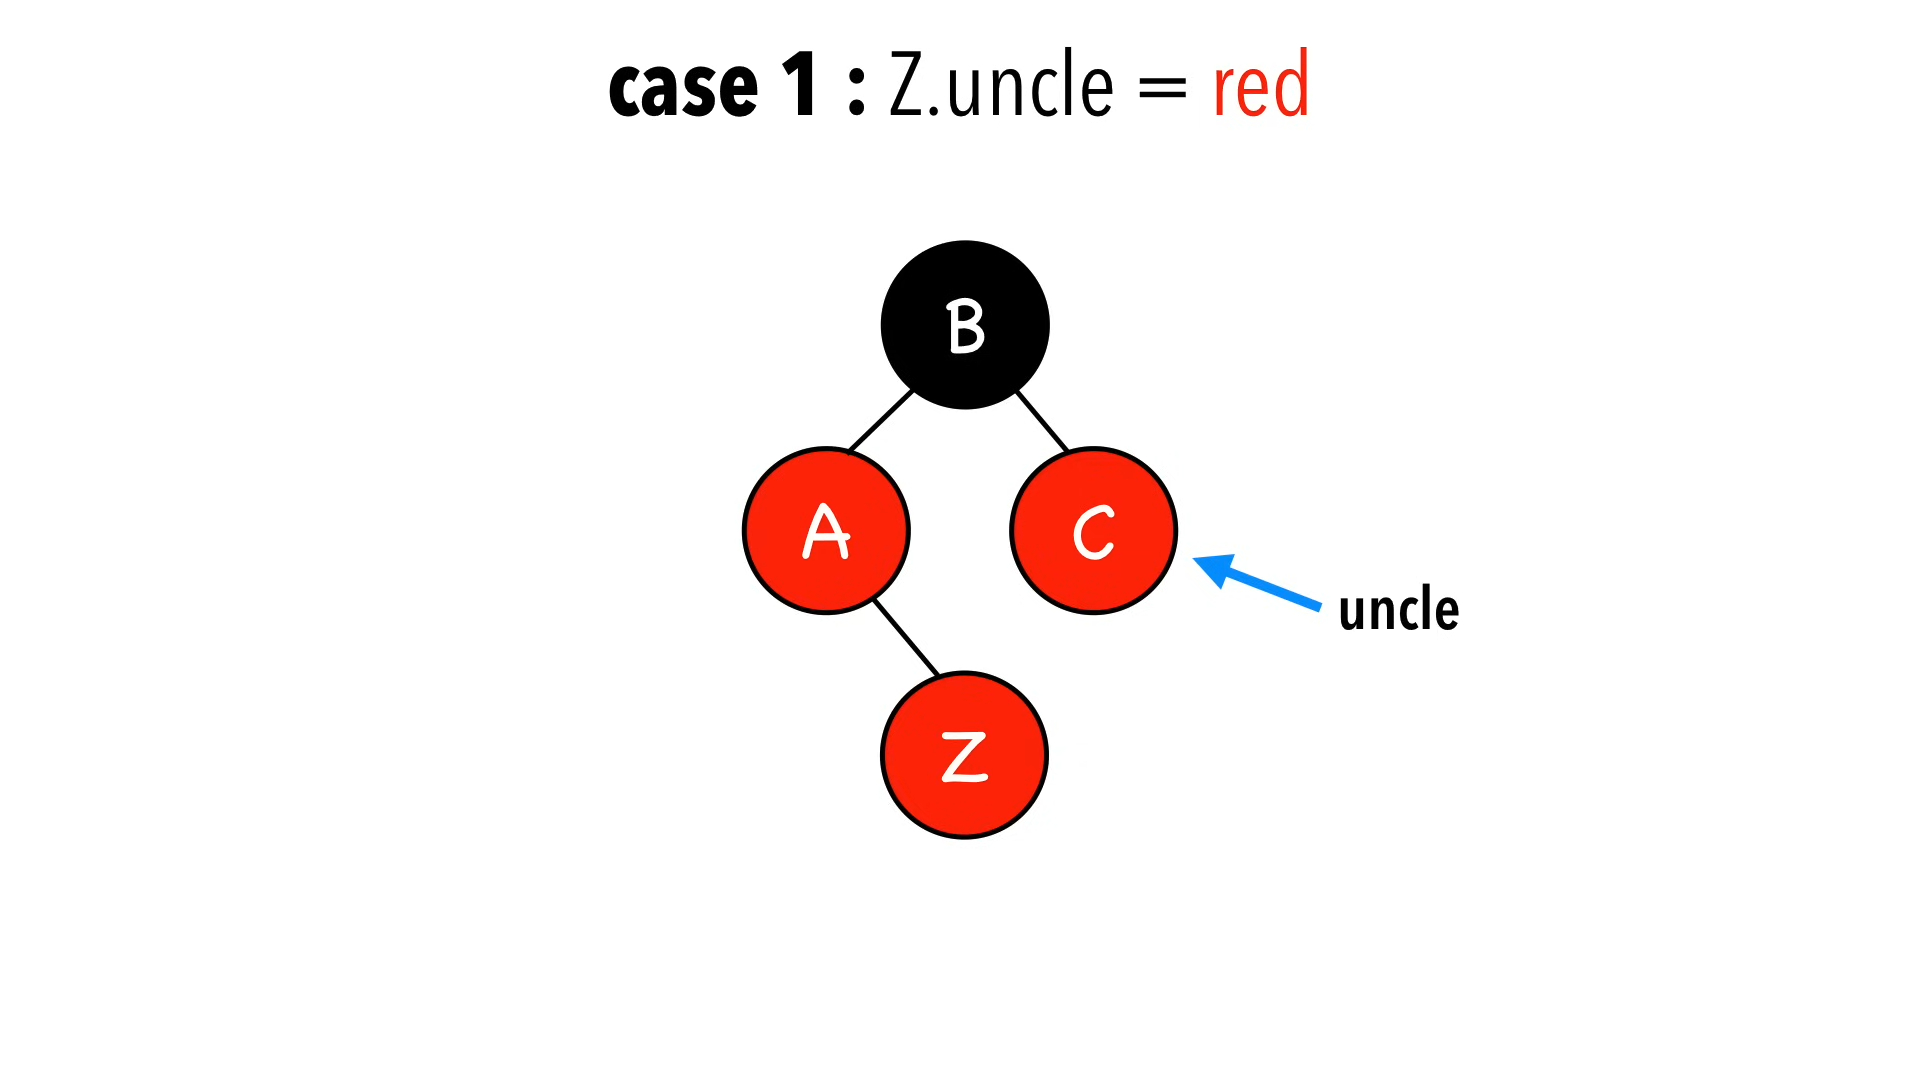
\includegraphics[width=0.45\linewidth]{images/rb-case-1-before.jpeg}
    \hfill
    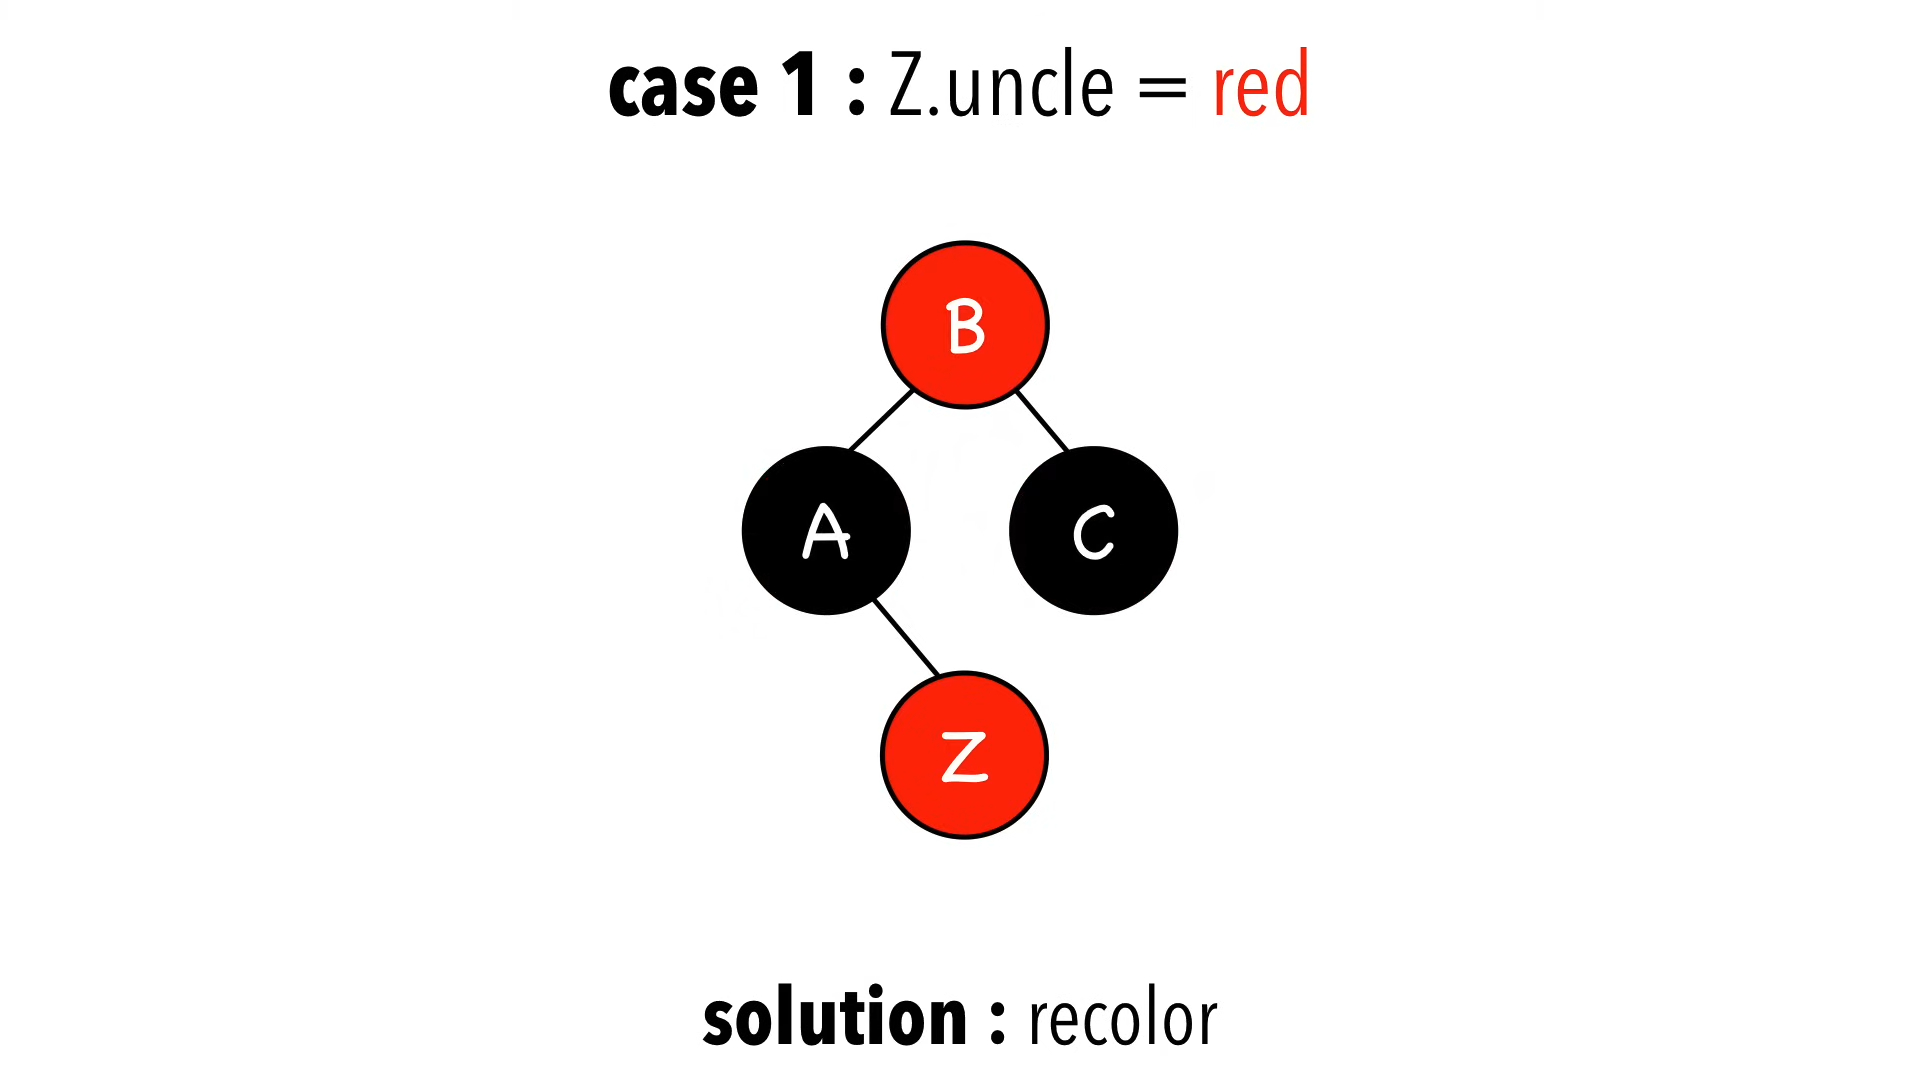
\includegraphics[width=0.45\linewidth]{images/rb-case-1-after.jpeg}
\end{figure}

\begin{figure}[H]
    \centering
    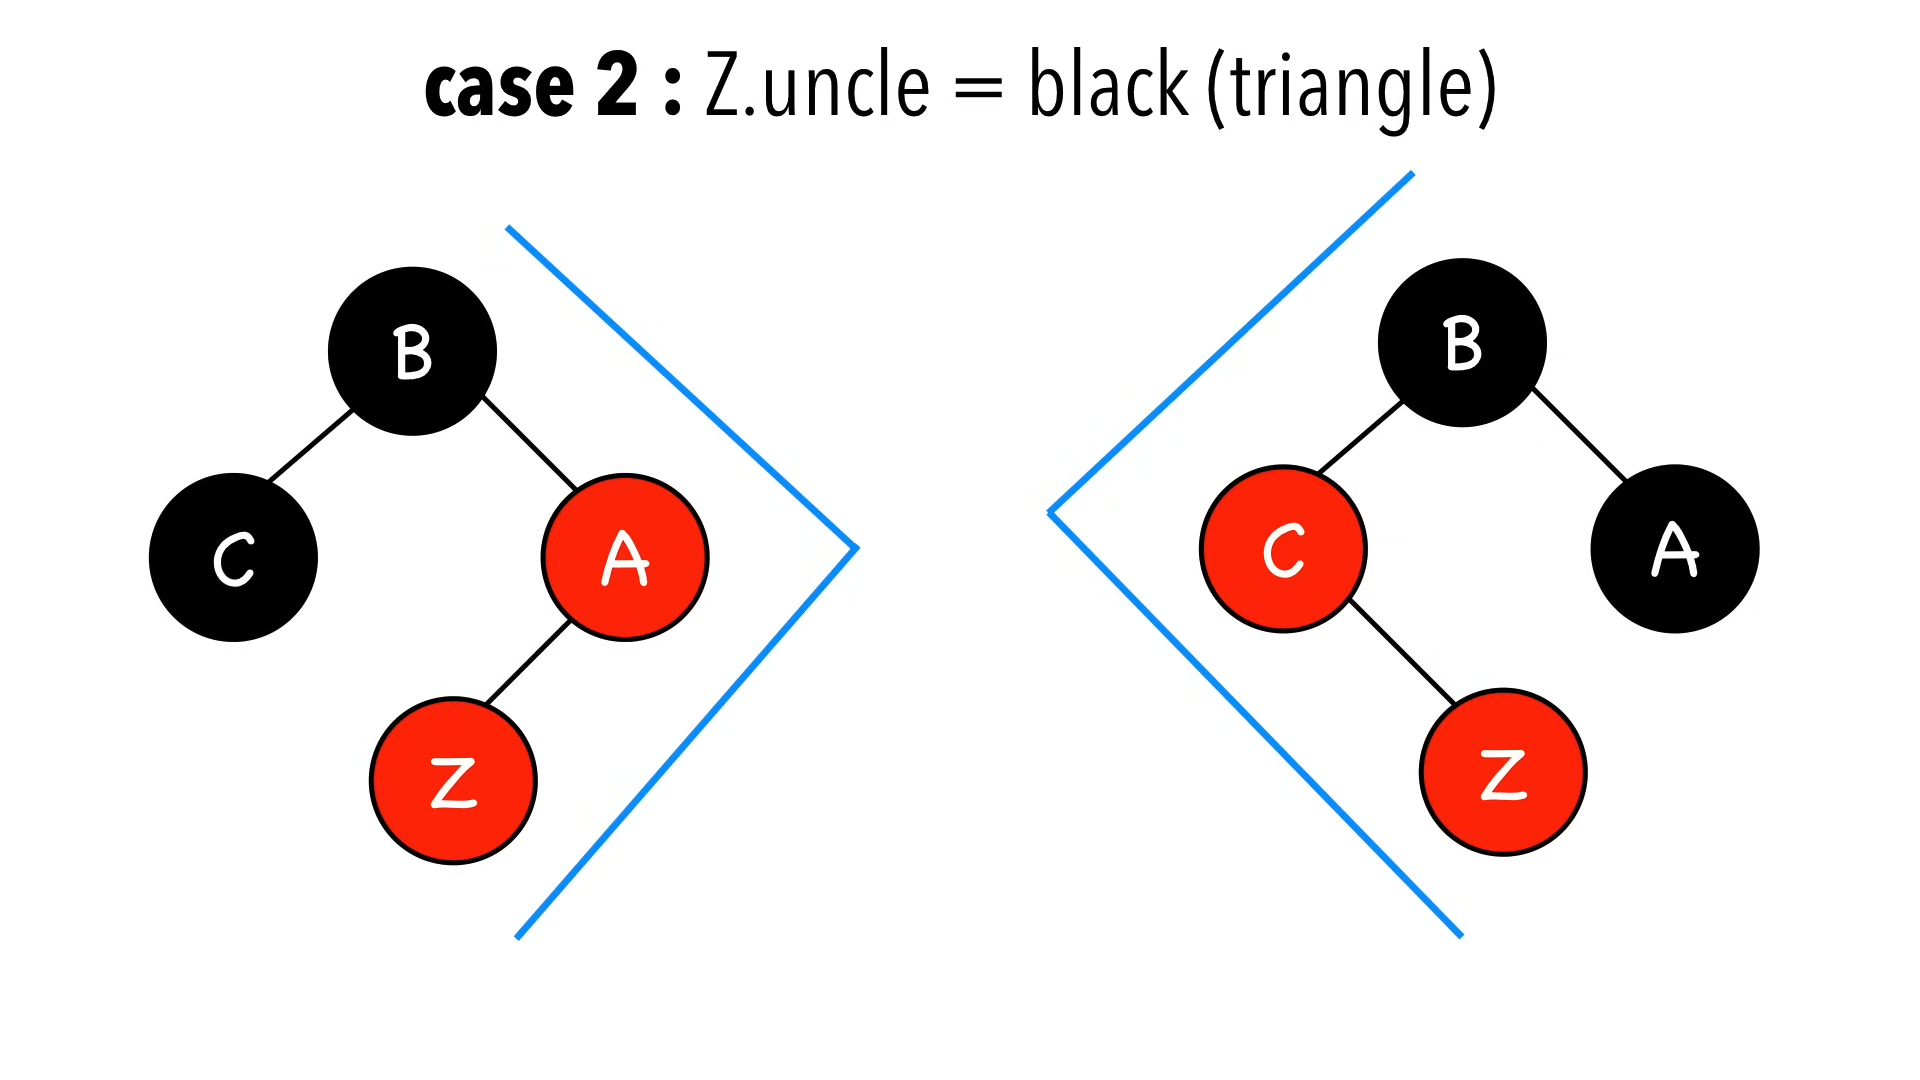
\includegraphics[width=0.45\linewidth]{images/rb-case-2-before.jpeg}
    \hfill
    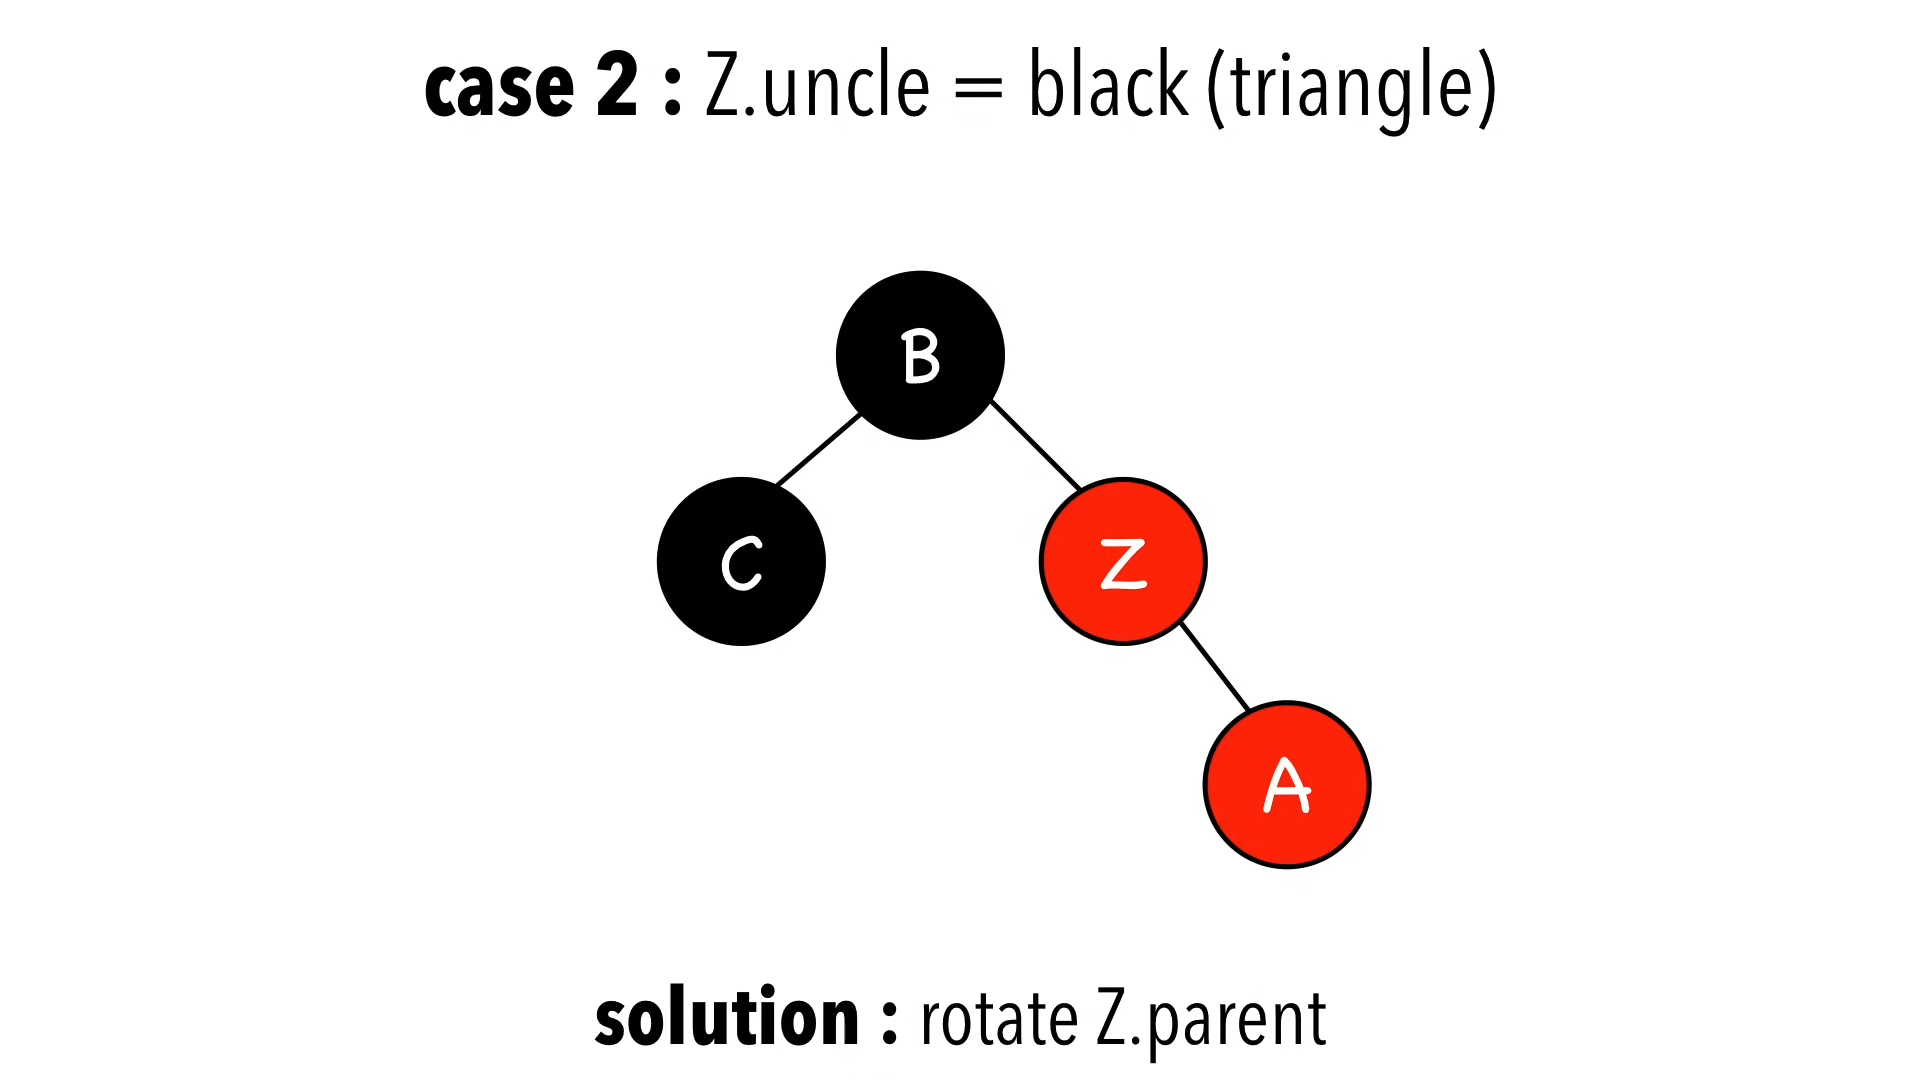
\includegraphics[width=0.45\linewidth]{images/rb-case-2-after.jpeg}
\end{figure}

\begin{figure}[H]
    \centering
    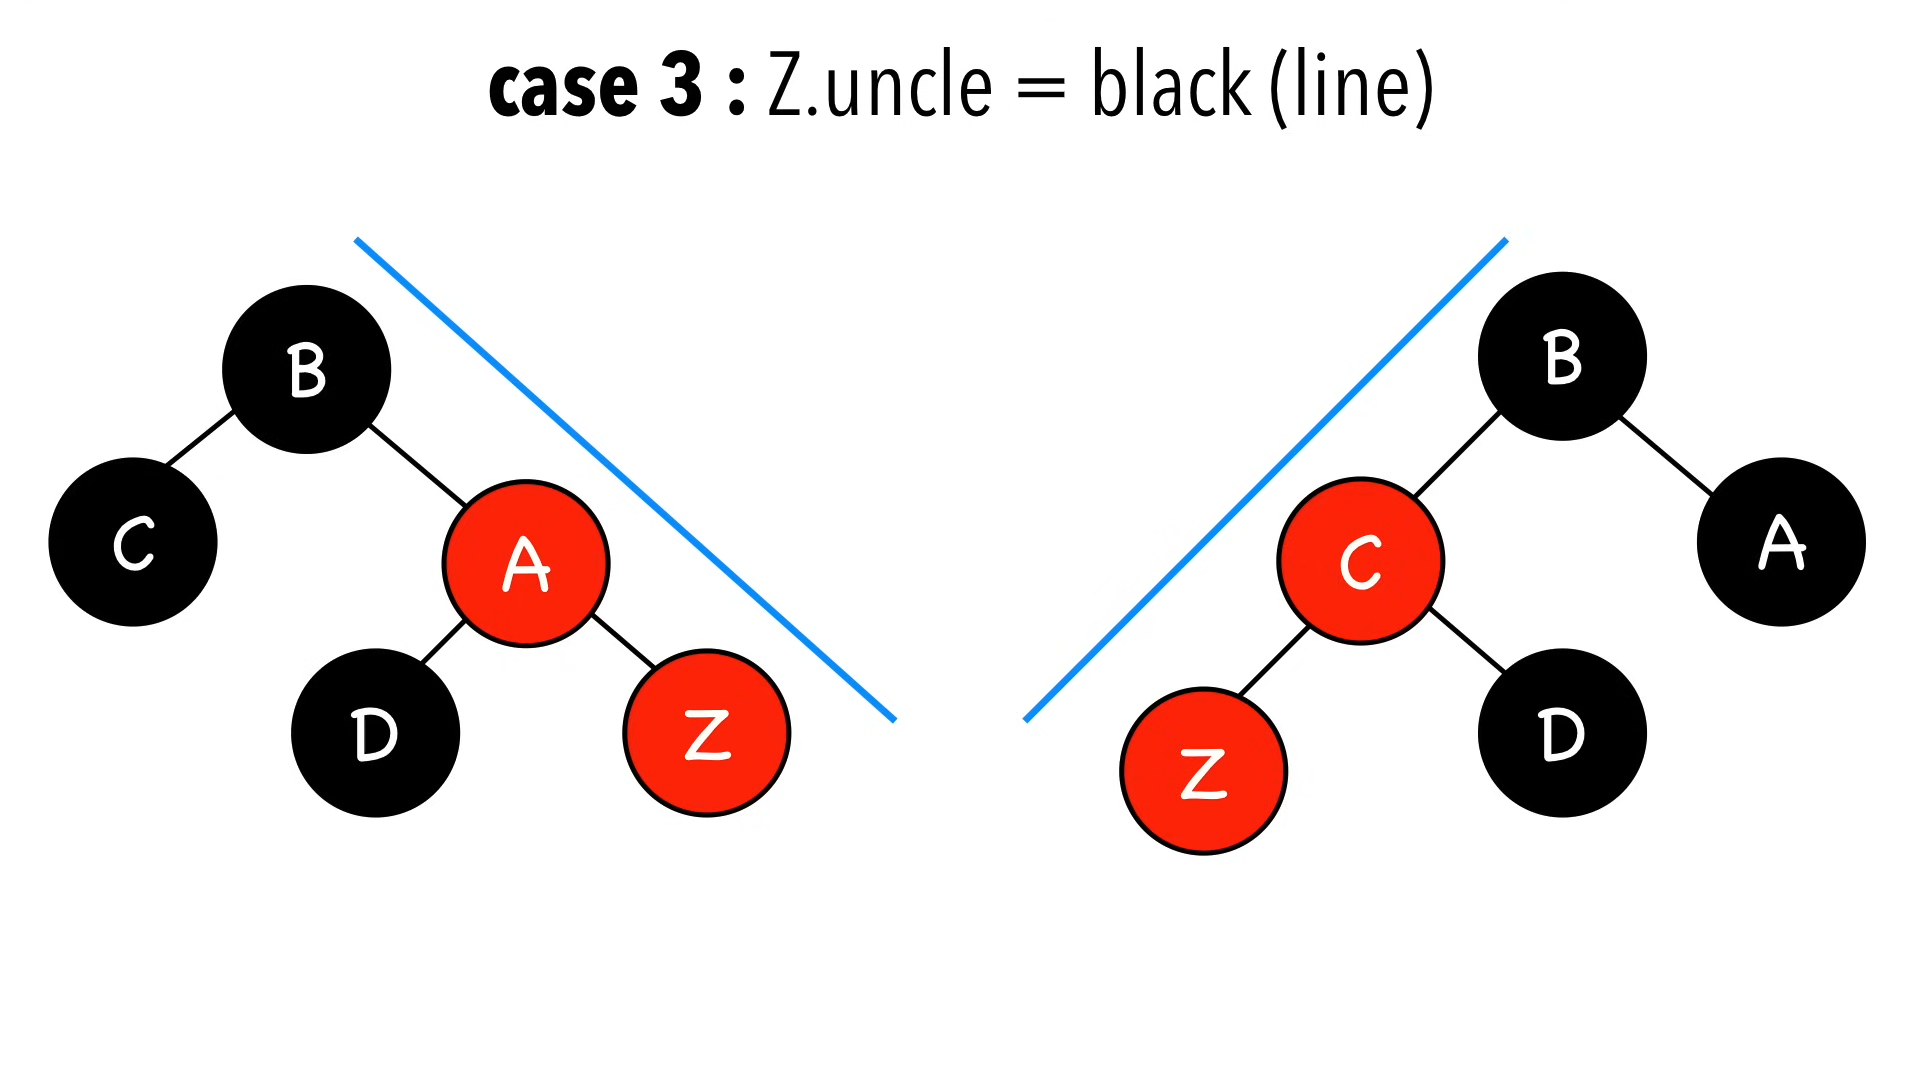
\includegraphics[width=0.45\linewidth]{images/rb-case-3-before.jpeg}
    \hfill
    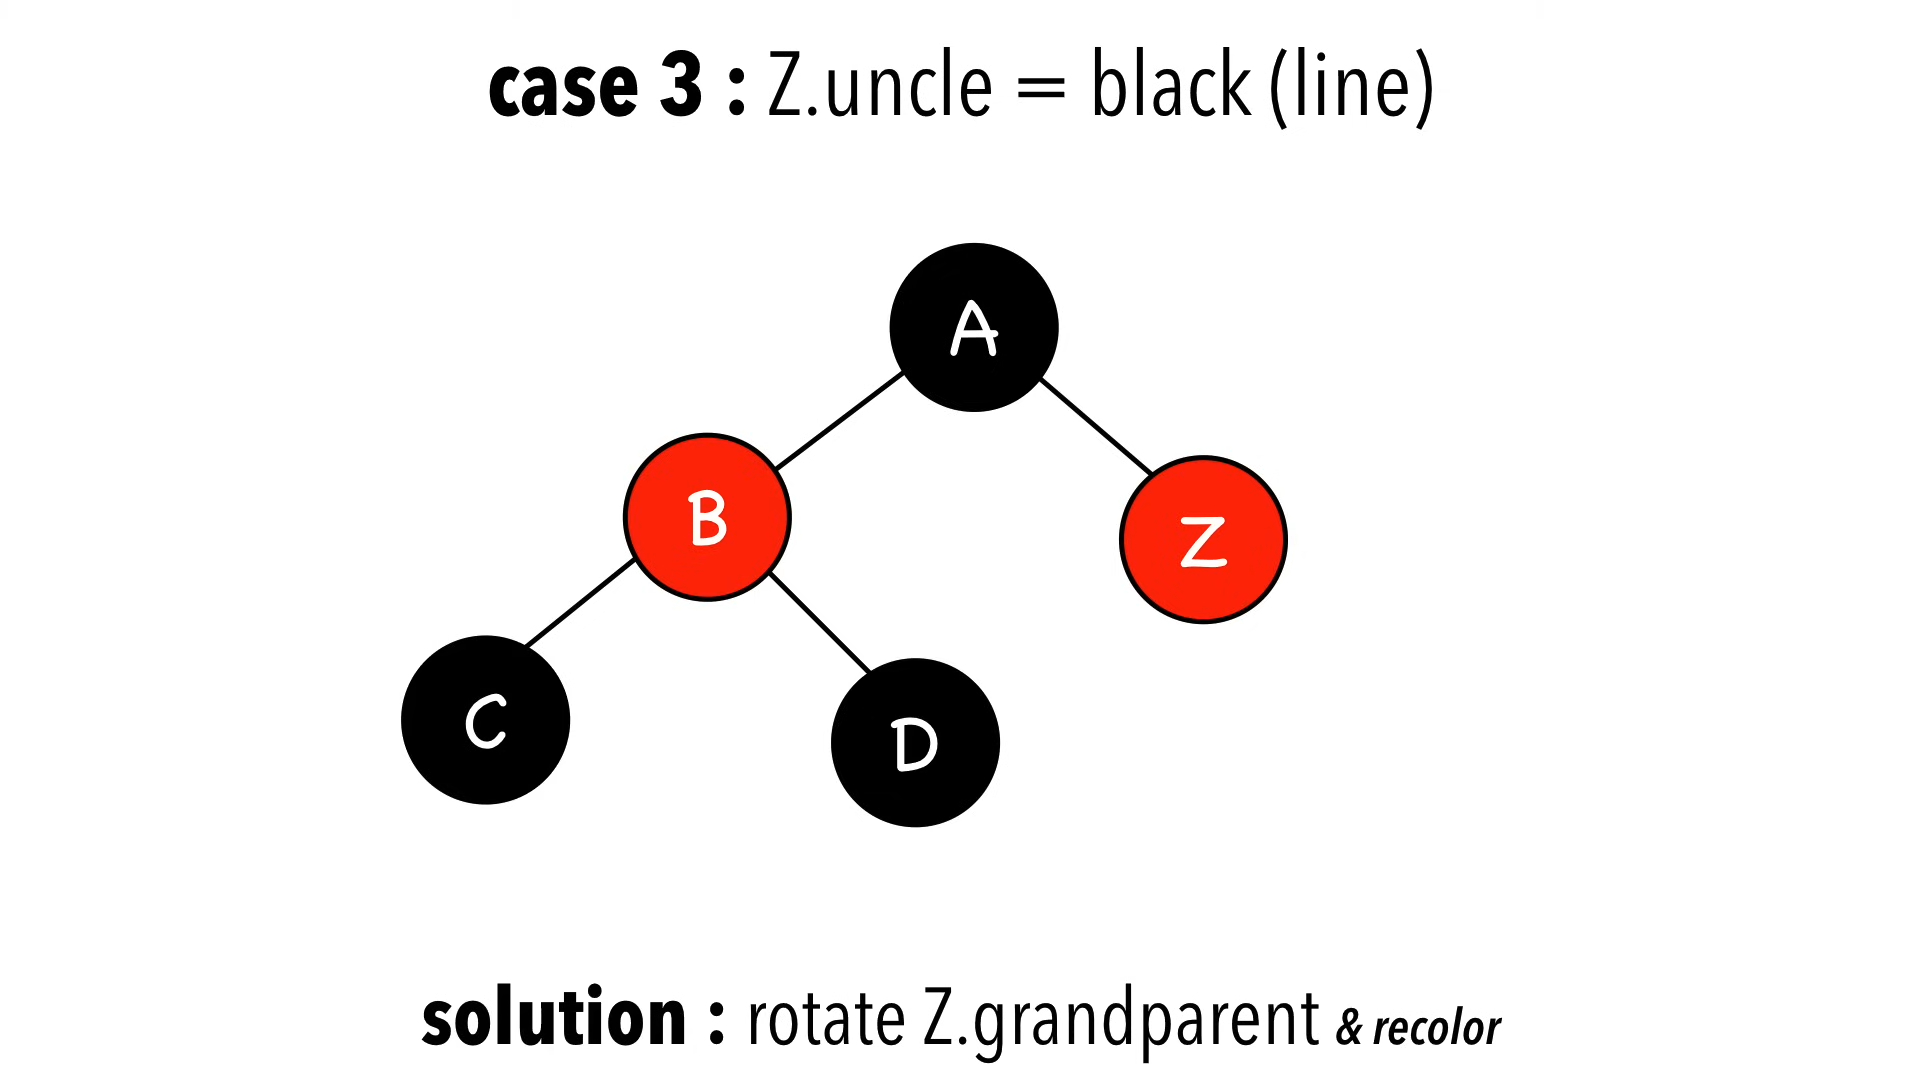
\includegraphics[width=0.45\linewidth]{images/rb-case-3-after.jpeg}
\end{figure}

\textbf{Important Note}: In this course, we use left-leading red-black trees, thus, if a node has only one red child, it must be the left child

\section{Graphs}

\textbf{Graphs are categorized into:}
\begin{itemize}
    \item \textit{Undirected graphs}: Edges are bidirectional.
    \item \textit{Directed graphs (Digraphs)}: Edges have a specified direction.
    \item \textit{Edge-weighted graphs}: Edges carry associated weights.
    \item \textit{Edge-weighted digraphs}: Directed graphs with weighted edges.
\end{itemize}

\textbf{Graph theory introduces:}
\begin{itemize}
    \item \textit{Path}: A sequence connecting a series of vertices.
    \item \textit{Cycle}: A path beginning and ending at the same vertex.
    \item \textit{Connected Components}: Isolated subgraphs where any two vertices are connected.
    \item \textit{Tree}: An acyclic connected graph.
    \item \textit{Bipartite Graphs}: Can divide vertices into two distinct sets with edges crossing between sets only.
\end{itemize}

\textbf{Important graph properties are:}
\begin{itemize}
    \item \textit{Eccentricity} of a vertex $v$: The greatest distance from $v$ to any other vertex. $e(v) = \max_{u \in V(G)} d(v, u)$
    \item \textit{Diameter} of the graph: The largest eccentricity of any vertex. $d(G) = \max_{v \in V(G)} e(v)$
    \item \textit{Radius} of the graph: The smallest eccentricity of any vertex. $r(G) = \min_{v \in V(G)} e(v)$
    \item \textit{Center} of the graph: Vertices with eccentricity equal to the radius. $C(G) = \{v \in V(G) \mid e(v) = r(G)\}$
    \item \textit{Girth} of the graph: Length of the shortest cycle. $g(G) =$ length of shortest cycle or $\infty$ if no cycles exist.
\end{itemize}

\textbf{For directed graphs:}
\begin{itemize}
    \item A \textit{directed graph}: A set of vertices connected by directed edges.
    \item \textit{Outdegree}: The number of outgoing edges from a vertex. \textit{Indegree}: The number of incoming edges to a vertex.
    \item Relationships in digraphs: No connection, one-way from $v$ to $w$, one-way from $w$ to $v$, or bi-directional.
    \item A \textit{directed path}: Follows the direction of edges. A \textit{directed cycle}: A path starting and ending at the same vertex without repeating edges or vertices.
    \item \textit{Reachability}: Key concept, differs from connectivity in undirected graphs due to directed paths.
\end{itemize}

\subsection{Graph Representations}
Graphs can be represented in various forms:
\begin{itemize}
    \item \textit{Adjacency Lists}: A list where each vertex stores a list of adjacent vertices, suitable for sparse graphs.
    \item \textit{Edge Lists}: A list of all edges. A second list of vertices may be necessary if this is used.
    \item \textit{Adjacency Matrices}: A 2D array where the presence of an edge between vertices is marked, ideal for dense graphs.
\end{itemize}

\subsection{Search Algorithms}

\subsubsection{Depth-First Search (DFS)}

\begin{enumerate}
    \item Create a set to keep track of visited nodes
    \item Add the current (or starting) node to the visited set
    \item For all neighbours of the current node, repeat 2 and 3
    \item Return the set of visited nodes, finish early if specific node found
\end{enumerate}

DFS ($O(V + E)$) will explore as far as possible before "backtracking", it can be implemented recursively or using a stack.

\subsection{Bredth-First Search (BFS)}

\begin{enumerate}
    \item Create a set to keep track of visited nodes, and add the starting node to it
    \item Create a deque, and add the starting node to it
    \item While deque is not empty:
    \begin{enumerate}
        \item Get next vertex by popping left from the deque
        \item For each neighbour of the next vertex, if it hasn't been visited, add it to the visited set and append it to the deque
    \end{enumerate}
    \item Return the set of visited nodes, finish early if specific node found
\end{enumerate}

BFS ($O(V + E)$) will explore all neighbours at the current depth level before moving to the nodes at the next level.

\subsection{Directed Graph Algorithms}

\subsubsection{Directed Cycle Detection}

Given a directed graph, check whether it contains a cycle or not.

\begin{minted}{python}
def detect_cycle(graph):
    # Helper function to perform DFS
    def dfs(node):
        # Mark the current node as visited
        visited[node] = True
        # Add the current node to the recursion stack
        rec_stack[node] = True

        # Iterate through all the neighbors of the current node
        for neighbor in graph[node]:
            # If the neighbor hasn't been visited, recursively call DFS
            if not visited[neighbor]:
                if dfs(neighbor):
                    return True  # Cycle found
            # If the neighbor is in the recursion stack, a cycle is detected
            elif rec_stack[neighbor]:
                return True  # Cycle found

        # Remove the current node from the recursion stack before backtracking
        rec_stack[node] = False
        return False  # No cycle found

    # Initialize visited array to keep track of visited nodes
    visited = [False] * len(graph)
    # Initialize recursion stack array to keep track of the current DFS path
    rec_stack = [False] * len(graph)

    # Iterate through all nodes in the graph
    for node in range(len(graph)):
        # If the node hasn't been visited, call DFS
        if not visited[node]:
            if dfs(node):
                return True  # Cycle found

    return False  # No cycle found
\end{minted}

\subsubsection{Topological Sorting}

\begin{itemize}
    \item A topological ordering is an ordering of the nodes in a directed graph where for each directed edge from node A to node B, node A appears before node B in the ordering
    \item The topological sort algorithm finds a ordering; they are not unique
    \item Not every graph can have a topological ordering. A graph which contains a cycle cannot have a valid ordering. Only Directed Acyclic Graphs (DAGs) have valid topological ordering
    \item All rooted tees have a topological ordering as they do not have any cycles
    \item Algorithm:
    \begin{enumerate}
        \item Pick an unvisited node
        \item Beginning with the first selected node, do a DFS exploring only unvisited nodes
        \item On the recursive callback of the DFS, add the current node to the topological ordering in reverse order
    \end{enumerate}
\end{itemize}

\subsubsection{Kosaraju's Algorithm}

\begin{minted}{python}
class KosarajuSCC:
    def __init__(self, G):
        # First pass: compute reverse postorder of reverse graph
        reverse_G = G.reverse()
        order = []
        visited = [False] * G.V
        for v in range(reverse_G.V):
            if not visited[v]:
                self.dfs(reverse_G, v, visited, order)
        
        # Second pass: find strong components
        visited = [False] * G.V
        self.id = [None] * G.V  # Component identifiers
        self.count = 0  # Number of strong components
        for v in reversed(order):
            if not visited[v]:
                self.dfs(G, v, visited, [])
                self.count += 1

    def dfs(self, G, v, visited, stack):
        visited[v] = True
        self.id[v] = self.count
        for w in G.adj[v]:
            if not visited[w]:
                self.dfs(G, w, visited, stack)
        stack.append(v)
\end{minted}

\subsection{Shortest Paths}

Understanding shortest paths requires comprehending several key properties and constraints:

\begin{itemize}
    \item \textit{Path Directionality:} Paths must follow the directed nature of edges.
    \item \textit{Weight Interpretation:} Weights may represent various metrics and aren't limited to physical distances.
    \item \textit{Reachability:} Some vertices might be unreachable from a given source, resulting in an undefined shortest path.
    \item \textit{Negative Weights:} These add complexity, especially when cycles are involved, potentially leading to undefined shortest paths due to infinite negative loops.
\end{itemize}

\subsubsection{Dijkstra's Algorithm}

Dijkstra's algorithm ($O((V + E) \log V)$, applicable to graphs with non-negative weights, proceeds as follows:
\begin{enumerate}
    \item Initialize the distance to the source to zero and all other distances to infinity.
    \item Set the source vertex as current and mark all other vertices unvisited.
    \item For the current vertex, consider all its unvisited neighbors and calculate their tentative distances through the current vertex. Update the neighbor's distance if smaller.
    \item Once all neighbors are considered, mark the current vertex as visited and select the unvisited vertex with the smallest tentative distance as the next current vertex.
    \item Repeat steps 3 and 4 until all vertices are visited.
\end{enumerate}

\subsubsection{Topological Sorting}

For directed acyclic graphs (DAGs), we can find shortest paths more efficiently:

\begin{enumerate}
    \item Perform a topological sort on the graph to order the vertices linearly.
    \item Initialize distances from the source to all vertices as infinite except the source itself, which should be zero.
    \item Process each vertex in topological order, updating distances to each vertex from the source based on the currently known shortest paths.
\end{enumerate}

\subsubsection{Bellman-Ford Algorithm}

This algorithm ($O(V \cdot E)$) offers a solution for graphs that may contain negative weight edges:
\begin{enumerate}
    \item Initialize all distances as infinite except for the source, set to zero.
    \item For each vertex, apply relaxation to all edges by updating the cost to reach each vertex from the source if a cheaper path is found.
    \item In the relaxing step, we
    \begin{enumerate}
        \item Add the distance to the from node to the edge's cost
        \item If this sum is smaller than the distance to the to node, we update the distance to the to node to be this sum
    \end{enumerate}
    \item Repeat the relaxation step for all vertices $V-1$ times, where $V$ is the number of vertices in the graph.
    \item Perform a final check for negative cycles by applying relaxation once more to all edges; if any distance is updated, a negative cycle exists. The check can also be repeated $V-1$ times, setting distances to all vertices reachable from negative cycles to $-\infty$. 
\end{enumerate}

\subsection{Minimum Spanning Trees}

\subsubsection{Kruskal's Algorithm}

$O(E \log E)$

\begin{enumerate}
  \item Sort all the edges of the graph by their weights.
  \item Initialize MST as empty.
  \item Traverse the sorted edge list:
    \begin{itemize}
      \item Add the current edge to MST if it connects two distinct components (no cycle is formed).
      \item Use the Union-Find data structure to check and manage components.
    \end{itemize}
\end{enumerate}

\subsubsection{Prim's Algorithm}

$O((V + E) \log V)$

\begin{enumerate}
  \item Initialize the MST with any single vertex, designated as the starting point.
  \item Repeat until the MST spans all vertices:
  \begin{itemize}
    \item Select the minimum weight edge that has exactly one endpoint in the MST.
    \item Add the selected edge and the adjacent vertex to the MST.
  \end{itemize}
\end{enumerate}

\textbf{Efficient Edge Selection:} The key challenge is quickly finding the minimum weight edge connecting the tree to any external vertex. This is efficiently managed using a priority queue.

\paragraph{Lazy Implementation}
In the lazy approach:
\begin{itemize}
  \item A priority queue (PQ) is used to lazily store edges with one endpoint in $T$.
  \item Edges are removed from the PQ until one with a valid external vertex is found.
  \item The process involves significant redundancy in edge consideration.
\end{itemize}

\paragraph{Eager Implementation}
In the eager approach:
\begin{itemize}
  \item Each vertex not in $T$ is associated in a PQ with the minimum weight edge that connects it to $T$.
  \item This setup reduces unnecessary operations and speeds up the algorithm.
\end{itemize}

\end{document}
